% Autor: Kryštof Glos

\chapter{Úvod}
Náhodně vytvářený obsah v herním průmyslu je velmi důležitou součástí her už po několik let. Mnoho her postavených na této vlastnosti už se prosadilo na trhu a stále více se uplatňuje. Náhodné vytváření obsahu se používá například na tvoření herních map, věcí v místnosti, skládání různých dopředu vytvořených místností tak aby vznikla jedinečná mapa, zkrátka skoro všude. 

Hlavním důvodem používání náhodně vytvořeného obsahu je možnost opakovaného hraní stejné hry, bez toho aby se stala nezáživná. V budoucnu se procedurální generování rozhodně neztratí a naopak se bude ještě více využívat. Cíl této práce je vytvořit jedinečnou 2D hru z pohledu z hora, která právě takové náhodné vytváření bude používat. Hra je o přežití a ovládání skupiny domorodců a nastolení míru na ostrově. V kapitole \ref{Teorie} je detailně popsáno náhodné generování a různé metody,v kapitole \ref{solution} je vysvětleno jaké způsoby budou nejlepší k řešení, jak byla práce naplánována a proč. V kapitole \ref{realization} je popsaný způsob jakým byla hra řešena, použité metody a jejich význam.

\chapter{Teorie} 
\label{Teorie}
Ve světě her jsou dvě možnosti jak přistupovat ke tvoření obsahu, jedním z těchto způsobů je tradiční nebo také mechanické. \hyperref[traditional]{Mechanické generování} je nejjednodušší, ale také nejpracnější. Další možností vytváření obsahu je pomocí metod implementující náhodné, nebo také \hyperref[procedural]{procedurální generování obsahu}. (anglicky Procedural Generation dále jen PG) PG je složitější na implementaci, avšak jakmile je implementované tak už žádné navrhování úrovní není třeba, takové úrovně však mohou mít chyby pokud nejsou správně ošetřeny. (například nedostupné místnosti, rostlina na vodě, atd.)

Hry které mají pouze dvě dimenze se nazývají 2D. (z anglického two dimensions) Je mnoho žánrů 2D her, RPG (role playing game) hry na hrdiny s příběhem, strategií, Co-op (kooperační) které jsou postavené na spolupráci více hráčů, survival (hry o přežití), colony-sim (z anglického colonization simulation) které mají simulovat kolonizaci ovládanou hráčem a tak dále. Tato bakalářská práce se zabývá hrou žánru colony-sim. Je mnoho způsobů jak vyvíjet takovou hru, nejčastěji se používají takzvané \hyperref[enginy]{herní enginy}, které takové vyvíjení hry ulehčují a jsou na to stavěné.


\section{Způsoby generování obsahu}
V této části porovnáme mechanické generování obsahu s procedurálním, vysvětlíme co je lepší kdy použít a jaké známe metody pro procedurální generování. Následující tři body popisují faktory, které je třeba zvážit při rozhodování, zda bude využita nějaká procedurální metoda na generování, nebo bude lepší použít manuální design úrovní a obsahu:
\begin{description}
	\item[Žánr tvořené hry] Při vytváření například takové FPS hry, u které záleží hlavně na ovládání a souboji hráče proti hráči, není třeba vytvářet mapy a další obsah procedurálně. Většinou stačí vytvořit například pouze jednu úroveň a na to není potřeba požívat procedurální generování. Při hrách které závisí na okolí, surovinách a přežití kde každá okolnost nějak ovlivňuje hráče, už procedurální generování hraje větší roli
	\item[Opakovaná hratelnost] Některé hry jsou dělané tak že čím déle hráč hraje stejnou úroveň(anglicky level) tím více se zlepšuje a je za to například odměňován je právě manuální tvoření úrovní lepší než procedurální. Naopak u jiných her, které mají úrovně procedurálně generované, většinou hráč danou úroveň zvládne, pokračuje na další a nepředpokládá se že se k ní bude ještě vracet.
	\item[Aspekt designu hry] Jestliže hra závisí z velké části na jedné úrovni s jejími mechanikami, vlastnostmi a obsahem, pak je lepší ji vytvářet mechanicky a doladit všechny vlastnosti a interakce s hráčem.
\end{description}


\subsection{Mechanické generování obsahu}
Tento typ generování lze dělat dvěma způsoby, jedním z nich je ruční tvoření
\label{traditional}
\todo{informace o tradičním generování obsahu}

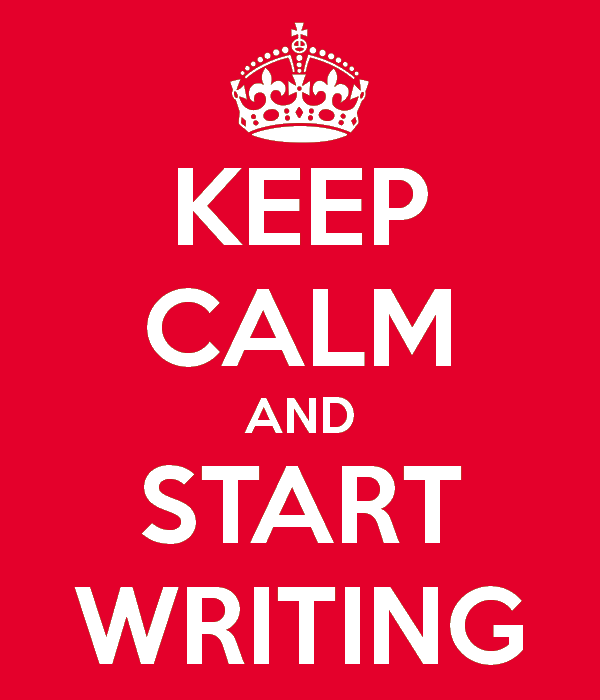
\includegraphics[scale=0.3]{obrazky-figures/keep-calm.png}

\textcolor{gray}{\blindtext[5]}


\subsection{Procedurální generování obsahu}
\label{procedural}
\todo{informace o procedurálním generování obsahu}

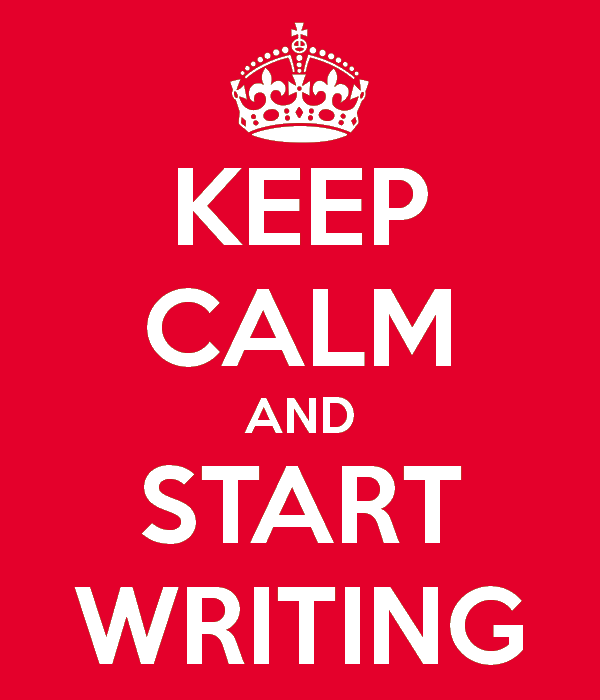
\includegraphics[scale=0.3]{obrazky-figures/keep-calm.png}

\textcolor{gray}{\blindtext[5]}


\subsubsection{Známé metody na procedurální generování}
\label{metody}
thsi is \cite{Short} aha
\todo{informace o všemožných známých metodách procedurálního generování}

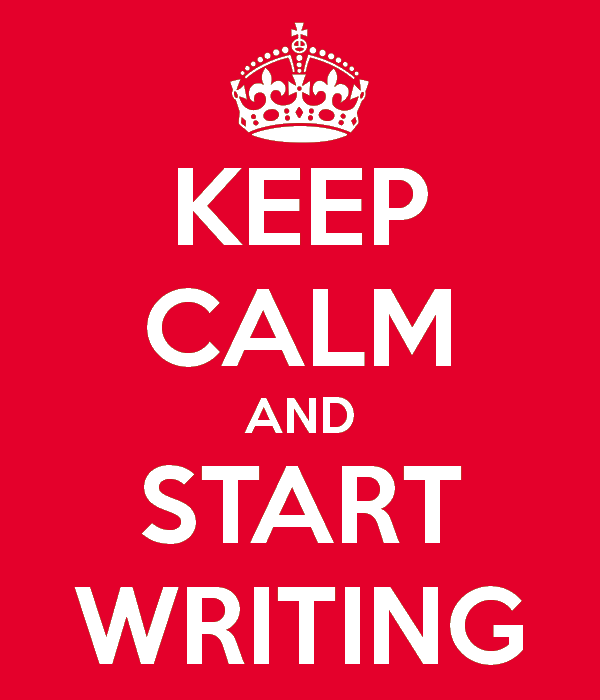
\includegraphics[scale=0.3]{obrazky-figures/keep-calm.png}

\textcolor{gray}{\blindtext[10]}


\subsubsection{Porovnání metod}
\todo{porovnání jednotlivých metod}
\textcolor{gray}{\blindtext[8]}

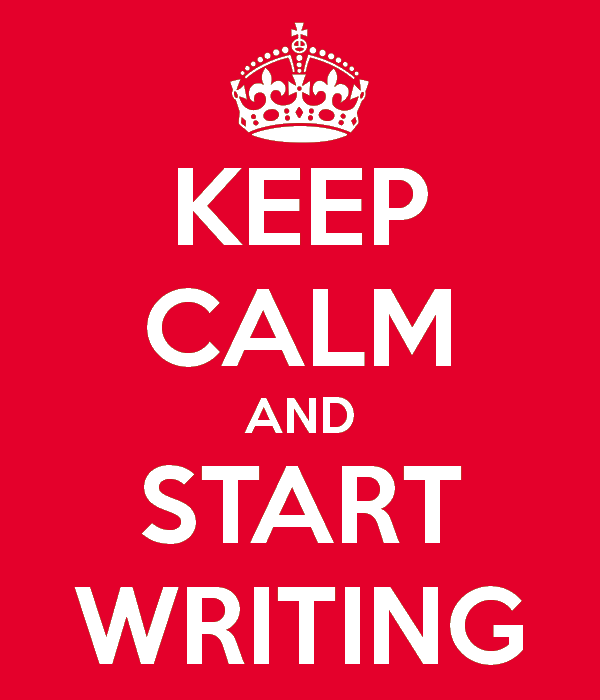
\includegraphics[scale=0.3]{obrazky-figures/keep-calm.png}

\textcolor{gray}{\blindtext[23]}


\section{2D hry}

\todo{popis hry}
\textcolor{gray}{\blindtext[18]}
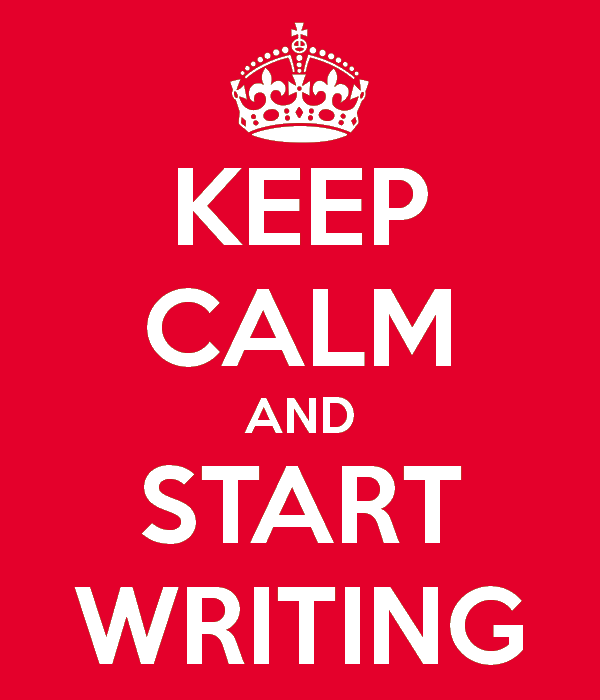
\includegraphics[scale=0.3]{obrazky-figures/keep-calm.png}

\subsection{Enginy na vývoj her}
\label{enginy}
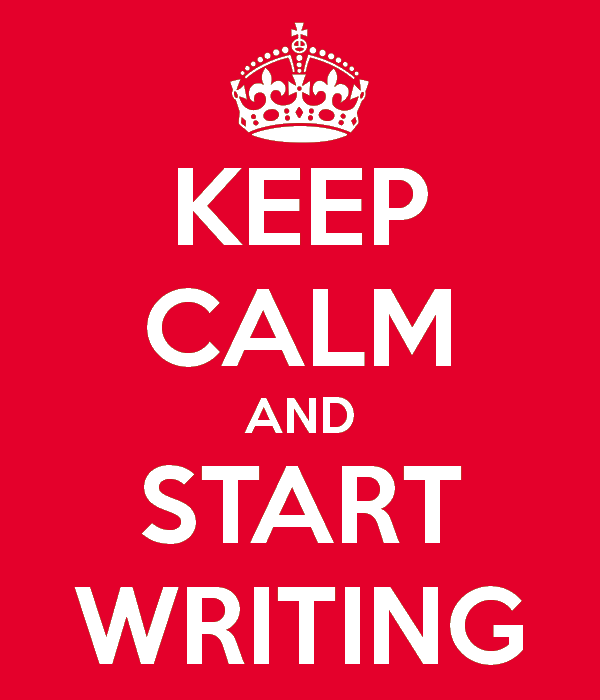
\includegraphics[scale=0.3]{obrazky-figures/keep-calm.png}

\textcolor{gray}{\blindtext[18]}

\chapter{Návrh řešení}
\label{solution}
\textcolor{gray}{\blindtext[2]}
\textcolor{gray}{\blindtext[46]}

\section{Vybraná metoda generování}
\todo{podrobnější popis metody, výhody, nevýhody}
\textcolor{gray}{\blindtext[46]}

\chapter{Realizace, experimenty a vyhodnocení}
\label{realization}
\textcolor{gray}{\blindtext[94]}

\chapter{Závěr}
\label{end}
\textcolor{gray}{\blindtext[4]}